\newpage

\section{Dynamo: Amazon's Highly Available Key-Value Store}

It's 2007 and Amazon's global e-commerce platform must remain ``always-on'' despite continual component failures—outages cost revenue and customer trust. To achieve this, Dynamo sacrifices strict consistency for low-latency availability:

\begin{Def}[Design Goals of Dynamo]
    \textbf{Dynamo} is a decentralized, highly available key-value store designed to:
    \begin{itemize}
      \item \textbf{Always-Writeable:} Never reject writes under partitions or node failures, deferring conflict resolution to the read path.
      \item \textbf{Incremental Scalability:} Scale out by adding or removing nodes without downtime or manual repartitioning.
      \item \textbf{Decentralized Symmetry:} No central coordinator, based on Consistent Hashing (\ref{sec:shard}).
      \item \textbf{Low-Latency Performance:} Dynamo provides its clients an SLA (Service Level Agreement) that under any load, it provides 
      a 300ms response 99.9\% of the time.
      \item \textbf{Eventual Consistency:} Allow temporary inconsistencies under failures, ensuring all updates reach replicas eventually.
    \end{itemize}
    \noindent
    \textbf{Consistency Model:} Weak Consistency, favoring availability over strict consistency.
  \end{Def}
  

  \noindent
  Next we discuss how it achieves this decentralized, highly available key-value store:

  \begin{Def}[Quorum System -- Gossip (Part 1)]

    A user's keys is hashed to a point on a 128-bit ring and mapped to an ordered list of $N$ nodes (the \textbf{preference list}). The first clockwise node, $N_i$, becomes the \textbf{coordinator}:
      
        \begin{itemize}
          \item \textbf{Writes}: Coordinator $N_i$ receives and sends \texttt{put(key,value)} in parallel to the next top $N-1$ replicas, waits for acknowledgments from any \underline{$W$ distinct replicas} (\textbf{including itself}), then returns success to the client.
          \item \textbf{Reads}: $N_i$ receives and sends \texttt{get(key)} to all $N-1$, returning success after $R$ nodes acknowledge the read. 
          \item \textbf{Conflicts}: Divergent data is reconciled via a vector-clock versioning history. If the vector clocks cannot be merged, \underline{it is left to the \textbf{client} to resolve.}
          \item \textbf{Quorum Condition}: Choosing parameters $R + W > N$, ensures $R$ and $W$ overlap, diminishing staleness.
        \end{itemize}

        \noindent
        Concretely, if key $k$ hashes to $A$'s segment, $A$ is the owner of $k$'s data. Any other server $N$ holds copies of $k$'s data, but is \underline{\textbf{not the owner}} (replica).
      \end{Def}
      
    
    \newpage 
    \noindent
    We'll call the below a turtle-back diagram; it illustrates the quorum system in a basic configuration:
    \begin{figure}[h]
        
        \centering
        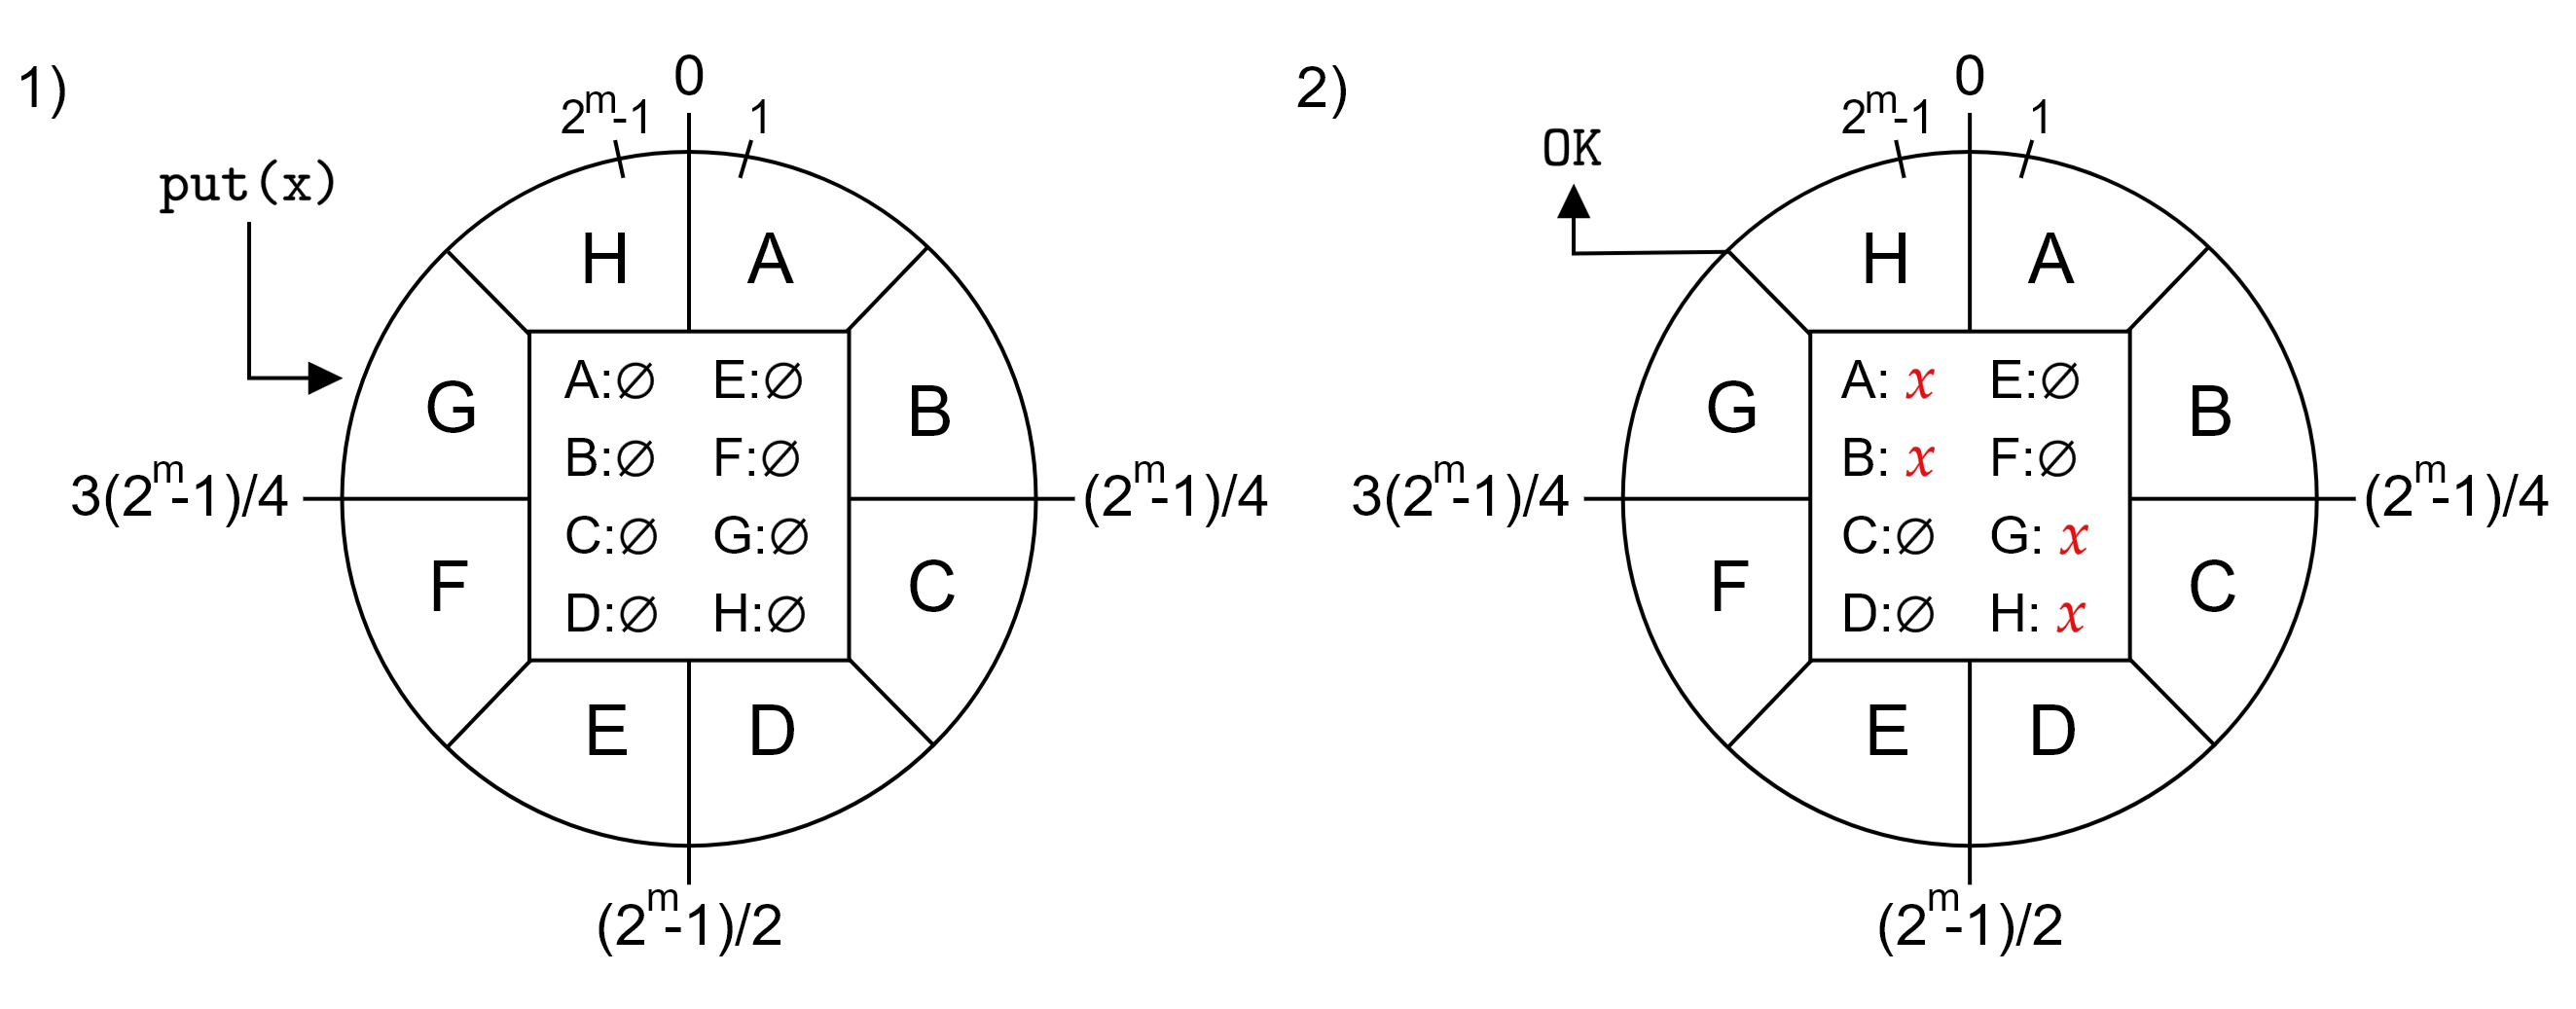
\includegraphics[width=\textwidth]{Sections/dyn/gossip.png}
        \caption{A basic quorum system. \textbf{To be clear}: virtual nodes are positioned at the spokes. For instance, \underline{$H$ starts at 0}, and ends at the next left-spoke $G$ (the top-left corner of the center box). Here, $R=4, W=4, N=7$, and servers are 
        an ordered list of virtual nodes $A$--$H$. Also, here we say \texttt{put(x)} for brevity, while it's actually \texttt{put(key,value)}.
        1) A client's put request falls within $G$'s range. 2) The next top $W-1$ nodes acknowledge, with $G$ sending back an \texttt{OK} (success).}
        \label{fig:quorum}
    \end{figure}

    \noindent
    Moving on, we deal with the liveness of nodes, and how to reconcile data:
    \begin{Def}[Quorum System — Gossip (Part 2)]

        Dynamo's monitors liveness with the following mechanisms:\\
      
        \noindent
        \textbf{Gossip Frequency \& Peer Selection:}  
        Every node, once per second, picks a peer uniformly at random and exchanges its local membership-change log. A vector clock represents the change log, where each cell is a (node, version) tuple.
        This random peer exchange ensures that knowledge of joins, leaves, and failures propagates exponentially fast without a central coordinator.\\
      
        \noindent
        \textbf{Failure Detection \& Sloppy Quorum:}  
        During a write, if a coordinator cannot reach a preferred replica (due to a failure or partition), it writes to the next healthy node in the preference list. That node stores the update alongside a \textbf{``hint''} tagging the intended replica.
        
        In particular, each node maintains hints stored in a separate log \underline{unbeknownst to the client}. The original paper makes no mention of any further constraints. This is called a \textbf{sloppy quorum}: it allows writes to proceed even if some replicas are unreachable.\\
        
      
        \noindent
        \textbf{Hinted Handoff:}  
        When the failed node rejoins, any node holding a hint for it will detect its revived liveness via gossip and then forward (“handoff”) the stored updates---restoring the full set of $N$ replicas \textbf{without} blocking client operations.
      \end{Def}

    \newpage 
    \noindent
    Below illustrates the gossip protocol and hinted handoff:
    \begin{figure}[h]
        
        \centering
        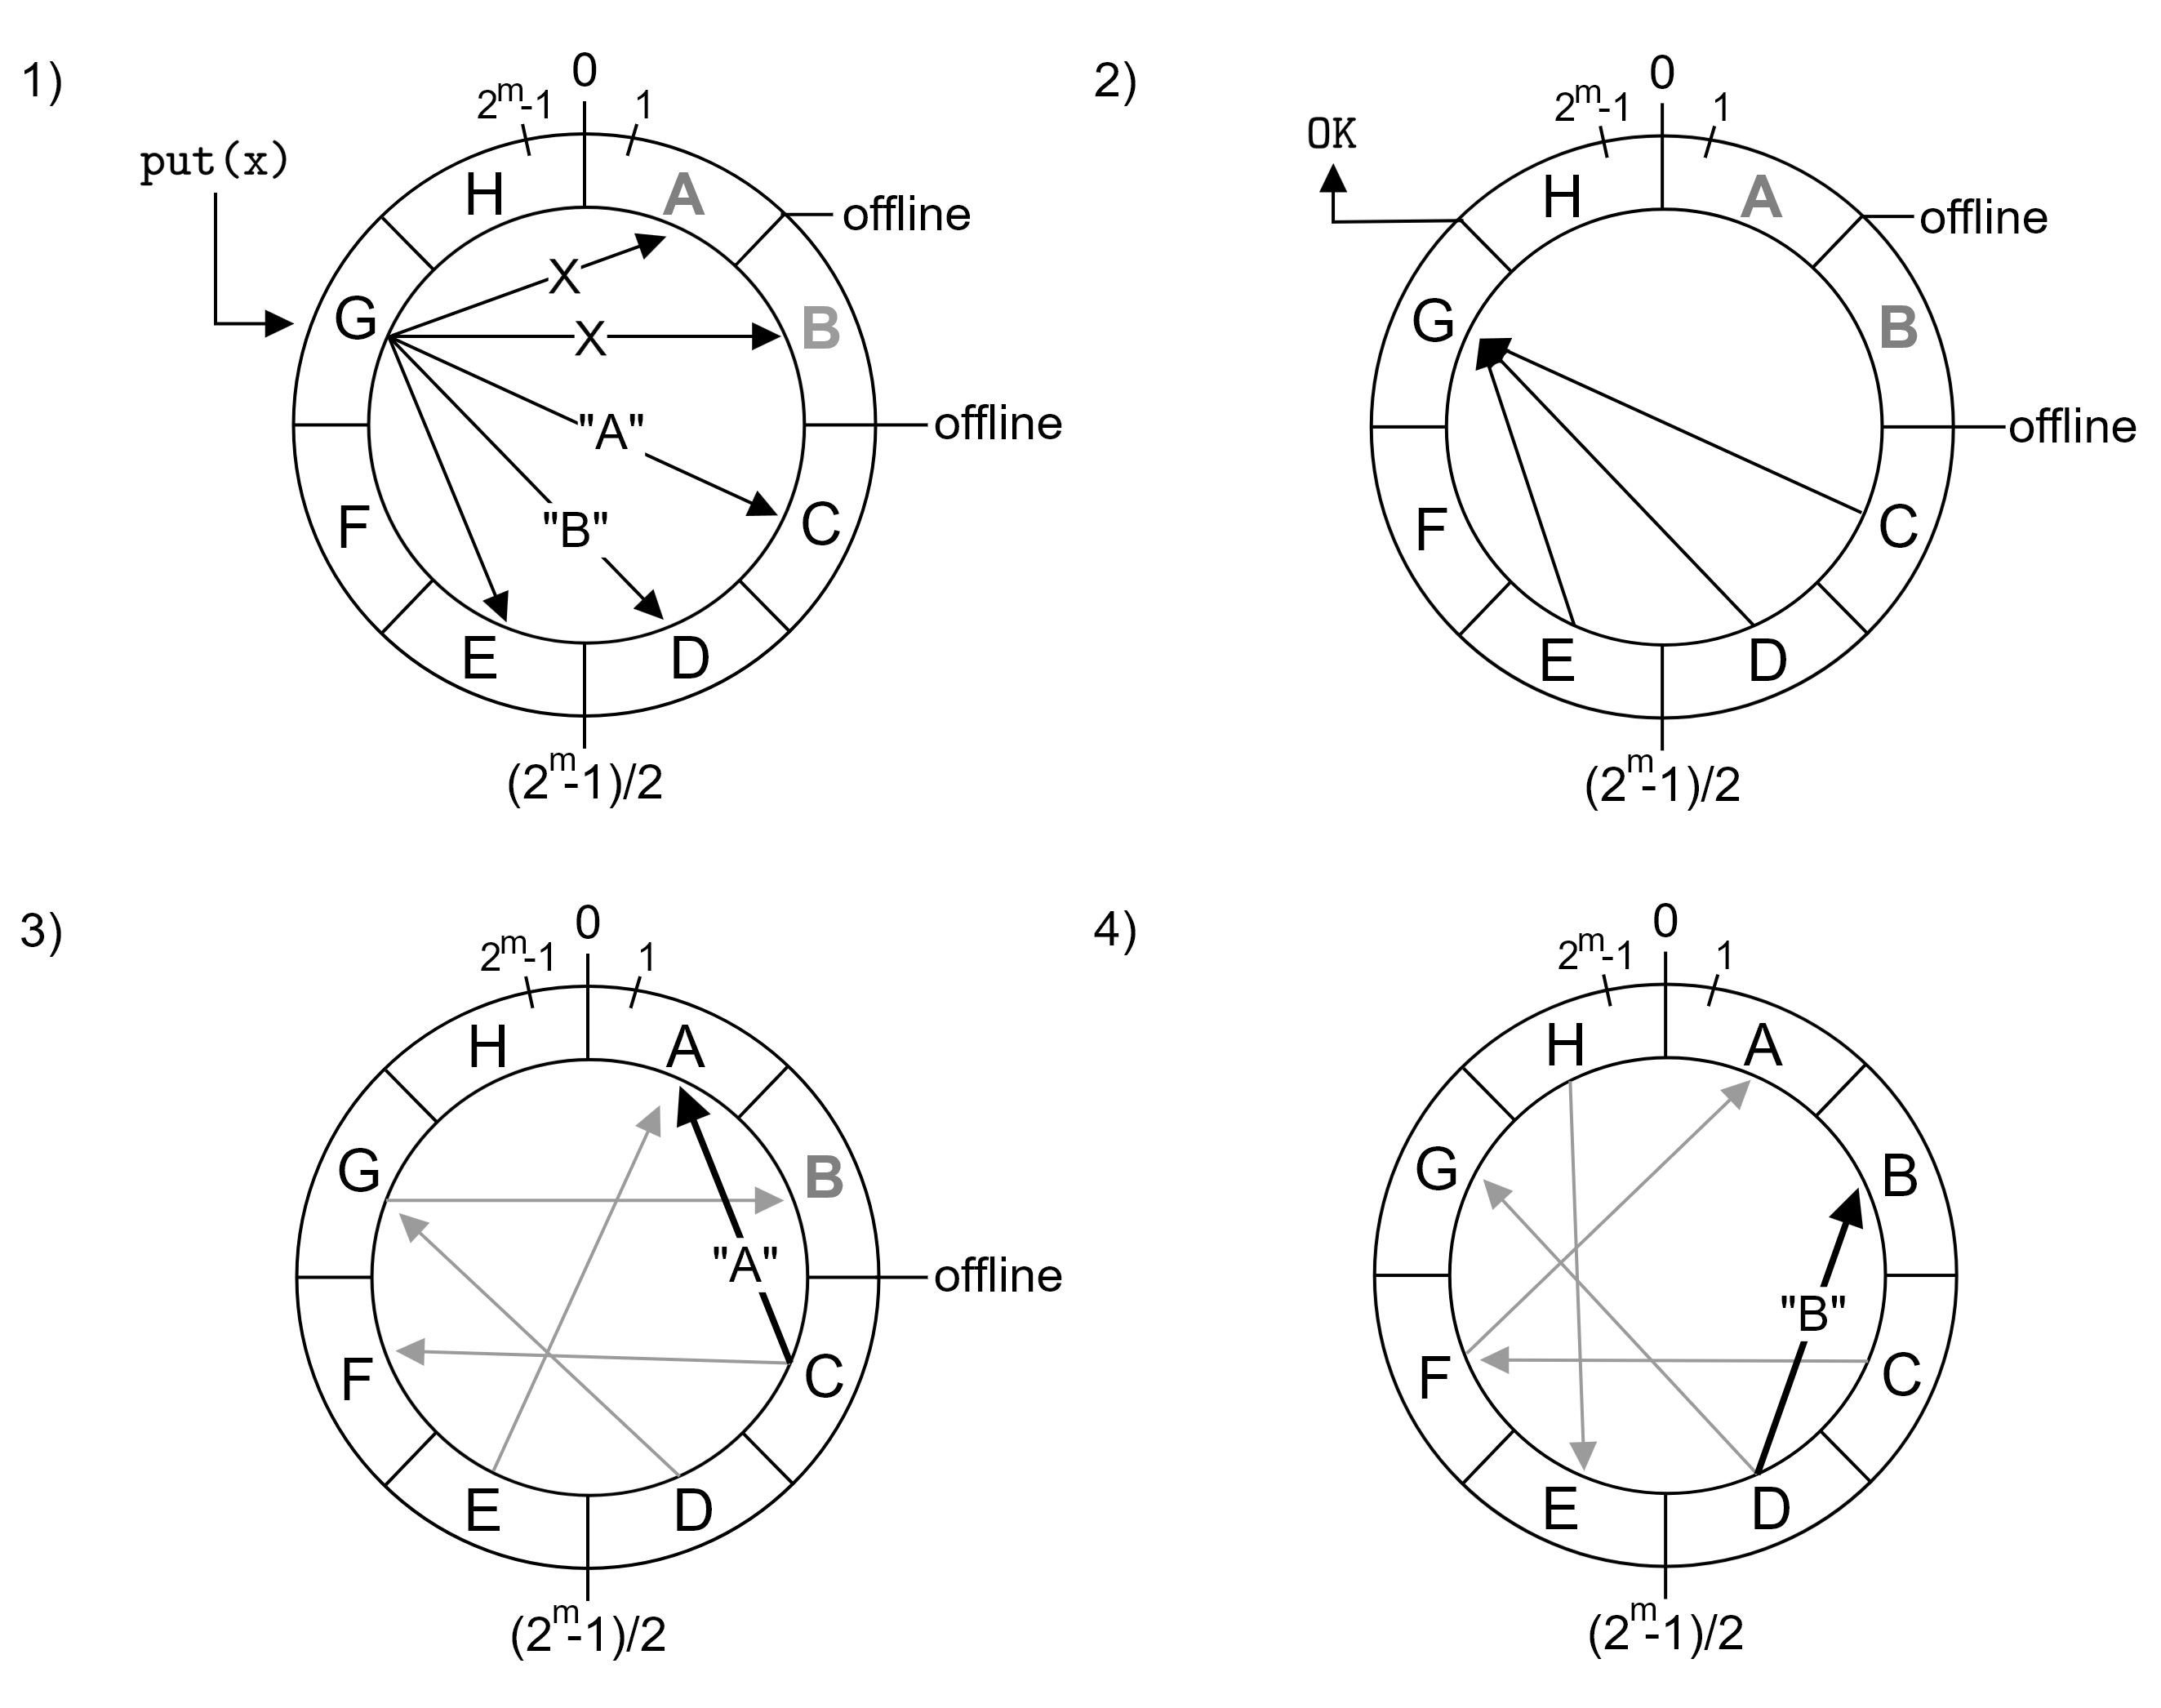
\includegraphics[width=\textwidth]{Sections/dyn/gossip_2.png}
        \caption{Gossip protocol and hinted handoff. 1) A put operation is sent to $G$, from which is then propagated. Though, $A$ and $B$ appear to be down, $G$ resolves this by giving hints to $C$ and $D$. 2) Nodes $C,D$ and $E$ \texttt{ACK}, allowing $G$ to return \texttt{OK}. 3) During the gossip protocol $A$ comes back online; $C$ notices this and sends the hint to $A$ (hinted-handoff). 4) Later in the 
        gossip protocol, $B$ comes back online; $D$ notices and hands off the hint to $B$. \textbf{Note}: The original paper doesn't specify whether a replica may only hold one hint or multiple hints. In this 
        figure we assume one hint per replica.}
        \label{fig:gossip}
    \end{figure}


    

%     \item \textbf{Sloppy Quorum \& Hinted Handoff:}  
%     To tolerate failures and partitions, reads and writes use the first $N$ reachable nodes in the preference list (“sloppy quorum”).  
%     Missing replicas receive “hints” that they eventually hand off when they recover.  
%   \item \textbf{Gossip-Based Membership:}  
%     Administrative join/leave events are written to a nod's local log.  
%     Every second, each node chooses a random peer to exchange (and reconcile) membership histories.  
%     This gossip protocol yields an eventually consistent view of which nodes are up, down, joining, or leaving, without any central coordinator.